%==================================================================================================
%   LUKES THESIS TEMPLATE 1.2
%   -------------------------
%   This template is based upon the offcial IMM PhD Thesis template, it is enhanced with a number
%   of new features and a number of errors have fixed. This template is intended to be complied to
%   PDF using PDFLATEX and is tested using the MiKTeX 2.9 LaTeX distribution.
%   It is based on the official DTU-IMM Thesis template by Finn Kuno Christensen in 2009.
%   Small bugfixes by Kasper Laursen in 2012 and 2013.
%   -------------------------
%   Last Updated: 2012-09-19
%   Contact: lthhe@imm.dtu.dk
%==================================================================================================
%
%==================================================================================================
% DOCUMENT SETUP
%==================================================================================================
\documentclass[10pt,twoside]{book}                  %Official DTU-IMM Thesis document setup
%
%Set to 'print' for printed version, use 'net' for online version
\def\thesisversion{print}
%
%==================================================================================================
% PACKAGES
%==================================================================================================
\usepackage{LukeThesis}                             %Import Thesis base style
\usepackage{hyperref}
%input{PhDMacros}                                   %Thesis specific macros
%
%==================================================================================================
% THESIS PROPERTIES (Modifiy these fields with your details)
%==================================================================================================
\def\thesisauthor{Brian Lynnerup Pedersen}          %Author
\def\thesistitle{Article Duplicates}		        %Title
\def\thesishandin{09-June}                          %Submission date (Day-Month}
\def\thesisdegree{B.Eng}                            %Degree ('B.Eng', 'B.Sc.', 'M.Sc.' or 'PhD')
\def\thesisyear{2014}                               %Submission year
\def\thesisnumber{????}                                 %DTU-IMM Serial number (do not include year)
\def\thesisISSN{0000-0000}                          %ISSN number
\def\thesiskeywords{Article Duplicates}  %PDF keywords
\derivethesisprops                                  %Derive dependent properties
%
%==================================================================================================
% SECTION NUMBERING SETUP
%==================================================================================================
\setcounter{tocdepth}{2}                            %2 adds sections up to subsections
\setcounter{secnumdepth}{3}                         %Subsubsections get a number when this is 3
%
%==================================================================================================
% THESIS STRUCTURE  (Modifiy to include more chapters etc)
%==================================================================================================
\begin{document}
%------------------------
%Pre-frontmatter material
%------------------------
\prefrontmatter
%--------------------
%Frontmatter material
%--------------------
\frontmatter
\pagenumbering{roman}                               %Set frontmatter numbering style
\chapter{Summary (English)}

The goal of this thesis is to document my work with implementing a working prototype of using algorithms to find article duplicates in a large corpus of articles. I will describe how the article inflow is currently working and how Infomedia plans on implementing my work in this inflow.

I will look at various algorithms for text comparison, and look into the possibility of creating my own algorithm or tweak an existing algorithm to better suit the needs for this job.

I will do an analysis of the task, and what kind of implementation I have done.

Finally I will write a summary of the work done, problems I have come across, and what the future of the project will be.                                   %English summary of Thesis
\markboth{}{}                                       %Set headings (left)(right)
\chapter{Summary (Danish)}
\begin{otherlanguage}{danish}

Målet for denne afhandling er at dokumentere mit arbejde med at finde artikel duplikater, i et større artikel corpus, ved brug af algoritmer. Jeg vil beskrive hvordan Infomedias artikel inflow virker nu, og hvordan Infomedia planlægger at bruge mit arbejde i fremtiden.

Jeg vil undersøge forskellige tekstsammenlignings algoritmer, og undersøge muligheden for at lave min egen algoritme, eller modificere en eksisterende algoritme til at bedre udføre det arbejde jeg laver i denne opgave.

Til sidst vil jeg gennemgå det arbejde jeg har lavet, hvilke problemer jeg løb ind i og hvad fremtiden for projektet vil være.

\end{otherlanguage}                                   %Danish summary of Thesis
\markboth{}{}                                       %Set headings (left)(right)
\chapter{Preface}

This thesis was prepared at the department of Informatics and Mathematical Modelling at the Technical University of Denmark in fulfilment of the
requirements for acquiring an M.Sc. in Informatics.

The thesis deals with ...

The thesis consists of ...
%==================================================================================================
% SIGNATURE AREA
%==================================================================================================
\vspace{20mm}
\begin{center}
    \hspace{20mm} Lyngby, \thesishandin-\thesisyear
    \vspace{5mm}
    \newline
  %Update signature image file in line below
    
\includegraphics[scale=0.5]{figures/SignatureDummy}
\end{center}
\begin{flushright}
    \thesisauthor
\end{flushright}
% % % EOF % % %                                     %Preface
\markboth{}{}                                       %Set headings (left)(right)
\chapter{Acknowledgements}

I would like to thank my supervisors from DTU, Inge Li Gørtz and Philip Bille, for the help they provided to my project. Also I would like to thank my company Infomedia, for letting me do my project for them, in particular my project leader Klaus Wenzel Jørgensen and Rene Madsen.


                            %Acknowledgements
\markboth{}{}                                       %Set headings (left)(right)
%------------------
% Table of contents
%------------------
\newpage\mbox{}\newpage
\chaptermark{Contents}
\pdfbookmark{\contentsname}{toc}
\renewcommand{\sectionmark}[1]{\markright{#1}}
\sectionmark{Contents}
\addtolength{\parskip}{-\baselineskip}
\tableofcontents
\addtolength{\parskip}{\baselineskip}
\renewcommand{\sectionmark}[1]{\markright{\thesection\ #1}}
%-------------
% Main content
%-------------
\mainmatter
\chapter{Introduction}
I have been working for Infomedia\footnote{\url{www.infomedia.dk}} since my third semester at DTU, studying as an IT engineer (BSc) at DTU (march 2012). Infomedia is in \underline{short} a company that deals with news monitoring.

Infomedia is the result of a fusion between Berlingske Avisdata and Polinfo in 2002, which means that Infomedia is partly owned by JP/Politikens Hus\footnote{\url{www.jppol.dk}} and Berlingske Media\footnote{\url{www.berlingskemedia.dk}}. It is a company with around 130 employees, of which a fair amount is student aides like myself. Infomedia has various departments, which includes an economy, sales, analysis and an IT department amongst others.\\
I am employed in the IT department as a student programmer.

Infomedia deals with news monitoring, which means that we have an inflow of articles\footnote{Articles are sent to Infomedia daily, this can be more than 40,000 articles per day.} from various newspapers, news sites, television and radio media, which we then monitor for content that is of interest to our clients. This can be a client that wishes to know when their firm is mentioned in the press or a product they are using, if that is being mentioned. Infomedia have also begun monitoring social media. Infomedia then sells various solutions to clients, for them to get this news monitoring.

One of the things that Infomedia tries to do, is that we want to present our clients with a fast overview of the articles in which terms\footnote{A term is, in short, a word or a combination of words. For the rest of my thesis a term will however only be a single word.}, that trigger our news monitoring, appear. Many local newspapers are today owned by bigger media houses (like the owners of Infomedia) and as such, they will feature a lot of the articles that have also been printed in the "mother paper". This will make the same (or roughly the same\footnote{Articles can be slightly edited in order to make them fit into the layout of the various papers.}) article appear many times in news monitoring. In an effort to make the list of articles presented to the clients, easy to look at, and preventing a client having to read the "same" article many times, Infomedia has a wish to cluster article duplicates. Infomedia can then present the client with a list of articles and in that list have further sub lists that contains duplicates of the original aritcle\footnote{Or the longest article rather, as this will tend to contain the most information.}. This also have an economic factor as clients are charged per article read.

Another issue, is the issue of copyrights and when the same article will appear in different media, but without content given from the author of that article. An example that is often happening is that news telegrams from Reuters\footnote{\url{www.reuters.com}} or Ritzau\footnote{\url{www.ritzau.dk}} is published in a newspaper, but without the source indication. All news media are of course interested in knowing when their material is being published in competing media. This how ever can be tricky business, as official rules on the matter is incredible fuzzy.

I will in this thesis try and look into various ways of identifying article duplicates within a test corpus\footnote{A days worth of articles from 10/31/2013 - totalling 22.787 articles.} of articles. The long term goal for Infomedia is having this being implemented in the inflow of articles, and having a look back functionality so that we can group duplicates not just for one day, but for a longer period of time. 
						%Chapter Introduction                             
\chapter{General - Terms and Rules}

I will in this chapter cover the essentials of the expressions and terms used throughout this thesis.

\section{Terms}

As there is a lot of terms used in this thesis, a short introduction to the most used are in order.
\begin{itemize}
\item \textbf{Article:} For this thesis, a digital document containing the contents of a piece of news. Could originate from papers, magazines, TV or other forms of media. For this thesis a document corresponds to an article. Articles are in their electronic form stored at Infomedia as XML files, I will throughout this thesis only deal with the part of the XML files that contains data of value to me in this assignment. This being \textit{Tags} (see below), \textit{Headline}, \textit{Sub headline} and \textit{Article Text}.
\item \textbf{Corpus:} From Latin meaning \textit{body}. In this thesis that describes the test set of articles being used a test set throughout my thesis.
\item \textbf{Monitoring:} In relation to the news monitoring (news surveillance) that Infomedia does, is the act of collecting news that holds information of value to our customers.
\item \textbf{Tag:} Used in Ontology\footnote{\url{http://en.wikipedia.org/wiki/Ontology_(information_science)}} to create words that describes the contents of an article.
\item \textbf{Term:} Basically a word. A term will be something that can be searched for.
\end{itemize}

\section{Matching}
I will in this thesis talk about false and true positives and negatives. A match will mean that two articles to some extend have the same content.

\begin{itemize}
\item \textbf{False Positive:} When an algorithm wrongfully identifies two articles as a match.
\item \textbf{False Negative:} When an algorithm wrongfully identifies two articles as not being a match, when in fact they are a match.
\item \textbf{True Positive:} When an algorithm correctly identifies two articles as a match.
\item \textbf{True Negative:} When an algorithm correctly identifies two articles as not being a match.
\end{itemize}


\section{Duplicates}
In this thesis I will often use the term 'duplicates' or 'match' about article comparisons. A duplication (match) can be an article that has been taken directly from a news feed and posted in a newspaper. Many local newspapers is owned by larger newspapers, and they will often receive articles from their owning paper. They will then print this in their own paper. Sometimes they will only use parts of the article and this will also be considered a duplicate for this thesis. As such duplication in this thesis is a way of describing how similar two articles are, rather than saying different papers are doing conscious fraud. That is a matter for another thesis.

\subsection{Topic Matching}
When looking at article matching, there is also the possibility of having articles score pretty well by the algorithms because they are dealing with the same topic. There are cases where the article have been heavily modified, and then there would be no basis to talk about duplication, then one could talk about topic matching. The article no longer contains the same phrases, but deals with the same topic.
Of course two articles could describe the same topic, but never have been related to begin with. I will not try and dissect whether this is the case, only try and indicate when I find two articles that are dealing with the same topic, and mark them as such. 

\subsection{Copyright}
It is hard to talking about duplicating without talking about copyrights. Although this thesis will not delve into whether something is duplicated as a part of a copyright infringement, it seems only reasonable to give a moment to talk about what a copyright is, and how it would affect duplication.

I feel that this quote is fulfilling as to explaining the concept of \textit{'copyright'}, even if it is talking about a case that is ongoing in USA at the time, and copyright rules can vary from nation to nation.
\begin{quote}
A copyright is basically a legal protection for an original expression on a fixed medium. So a song on a record, words on a page, ballet steps written down, and paint on a canvas are all copyrightable things. A phone book is not copyrightable (it’s not original). A copyright only protects the expression and not the underlying idea. Marvel does not have a corner on men in mechanical suits who fight crime – they only have the particular expression of that idea in Iron Man comic books.

Confused? That's okay. Copyrights are pretty complex things. A lot of what can be copyrighted is figured out in court when people fight over it. The basic test that the court will pose in this case is “is the expression original? Does the potentially infringing work actually borrow from the original expression?” ~\cite{Copyright}
\end{quote}

So the whole concept is extremely fuzzy, and often the infringement part will have to be settled in court. In the recent years that have been a lot of debate in which university educated people have become accused of plagiarism  in relation to their doctoral or master thesis\footnote{\url{http://www.theguardian.com/world/2011/feb/16/german-defence-minister-plagiarism-accusation}}$^{,}$\footnote{\url{http://www.nytimes.com/2012/04/03/world/europe/hungarian-president-pal-schmitt-resigns-amid-plagiarism-scandal.html?_r=0}}. A hard topic to deal with in a fixed way, and to top it off, there is also the notion of \textit{"fair use"}\footnote{\url{http://www.umuc.edu/library/libhow/copyright.cfm\#fairuse_definition}}. Although there is no real fair use paragraph in Danish law, we instead have \textit{'låneregler'}\footnote{\url{http://da.wikipedia.org/wiki/Fair_use}}. 

In the world that Infomedia is dealing with, articles are also a target of duplication, and a lot of effort have begun being invested into this, as it can be a question about a lot of money if you fail to protect your copyrighted material. So the motivation in finding article duplicates can be two sided. First off, it creates a better overview for Infomedia's customers, secondly newspapers are very interested in finding out if their material is being used, unlicensed, in other media.




Hvornår er en artikel et duplikat (korte artikler (breaking news), hvornår er to artikler "tilstrækkeligt" forskellige?)
blah about copyright rules in Denmark... 									%Chapter 2
\chapter{Analysis}

This chapter describes the considerations taken in picking an algorithm, as well as what is already implemented at Infomedia.

\section{Algorithms in General}
Before any sort of work can be done, one must consider various algorithm to work with. There are several text matching algorithms available for free on the Internet, and if one has the money for it, there are companies that can develop a specialized algorithm for you. As I do not have a lot of money (and paying for someone else, to do an algorithm for me, kind of defeats the purpose of this whole thesis) I have gone with the first option and found a free basic algorithm on the Internet, as well as contemplated to create my own algorithm from scratch.

\subsection{Requirements Analysis}
The algorithms should be able to live up to the following demands:

\begin{itemize}
	\item The algorithm should be able to work with text.
	\item Performance is of secondary importance, but should have good accuracy (performance < accuracy).
	\item The algorithm shall be able to return a score based on how identical two articles are.
	\item The algorithm should be focus on doing one thing only (not try to do several forms of text comparisons).
	\item The algorithm shall be available in an open source, or free to use, licence.
\end{itemize}

\section{Initial Considerations}
Infomedia already have an algorithm implemented in the inflow to make a rough comparison of the articles coming in. How ever, the thought is that a combination of several algorithms would provide a better and more granular view of the articles as they are being compared. A new algorithm should be one that was specialized in text matching. It should also be an algorithm that would work in different manner than what Infomedia already have implemented\footnote{More on the algorithm already implemented in the next section.}, as having two algorithms that work in more or less the same fashion would not produce results of much interest.

As the current implementation is rather fast, it could prove useful to have the algorithm that is already implemented, do the initial rough split of matches and no matches, and then have a slower (but more thorough) algorithm look at the \textit{interesting} article comparisons. Initially I have looked at two algorithms to fill this need, \textit{Longest Common Substring} and \textit{Semaphore Tag Matching} - an algorithm I would make from scratch.

\subsection{System Architecture}
As mentioned the various algorithms should work in different ways, meaning they should have various ways. This is to ensure a balanced image of how much an article comparison is actually a match. The thought is, that instead of having a few algorithm having to have many focus areas. It is better to have many that only focus on one thing, then combine their scores into a broad representation of how similar two articles is.

\pagebreak

\begin{figure}
	\centering
	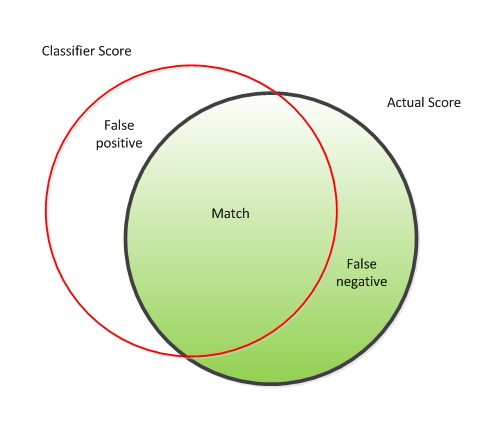
\includegraphics[scale=0.5]{figures/SingleAlgoScore}
	\caption{Variation between how a single algorithm might score an article comparison, and how the actual score should be\cite{Slides}.}
\end{figure}

The essential thing in this, is to ensure that the various algorithms works in different ways. If one were to use many algorithms that all focused on the same way of doing text comparisons, the results would not provide that broad image of scores that is wanted for a more accurate score representation.

\begin{figure}
	\centering
	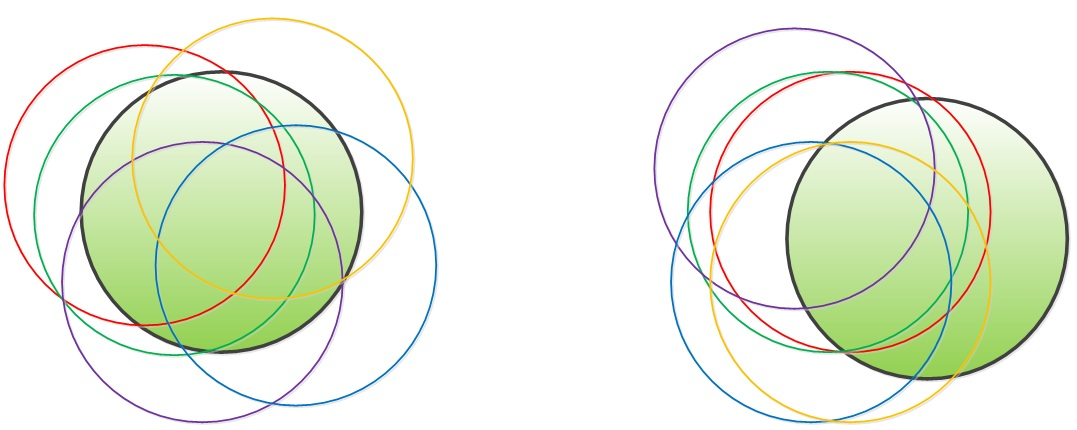
\includegraphics[scale=0.3]{figures/MultipleAlgoScores}
	\caption{\textbf{Left:} A balanced score, obtained by using several algorithm with different focus areas. \textbf{Right:} An unbalanced score, obtained by using several algorithms with the same focus area\cite{Slides}.}
\end{figure}

The idea is that the algorithms should do 99.9\% of the work in identifying article duplicates, and then have the  last 0.1\% be verified by humans. This is already how things are working at Infomedia, but only with one algorithm at the moment. My work will the be the first algorithm to do a check of the work done by the already implemented algorithm. This will hopefully narrow the field of possible article duplicates that has to be verified by human eyes.

The system would then ideally work as follows.

\begin{figure}[h]
	\centering
	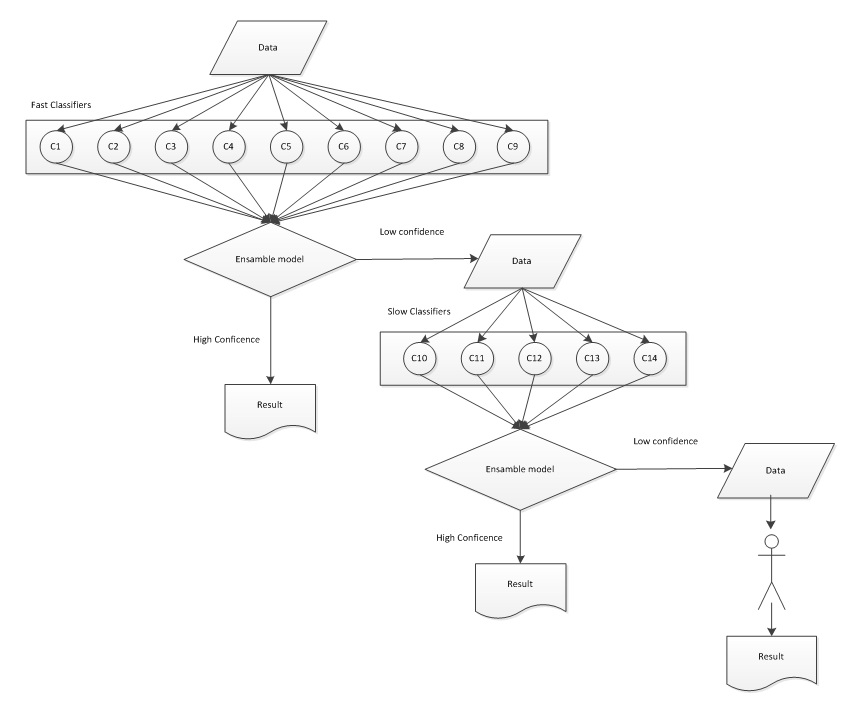
\includegraphics[scale=0.5]{figures/SystemArchitecture}
	\caption{System Architecture, with many algorithms doing text analysis\cite{Slides}.}
	\label{Architecture}
\end{figure}

When data (articles) arrives in the inflow, a number of fast algorithms would then do the rough split of the comparisons. All of these comparisons would then receive scores, that would then be evaluated through the ensemble model. If the scores leaves no doubt (is over a given threshold) that the article comparison is a match, the comparison would stored as a match. If the scores of the comparisons leaves some degree of doubt as to whether a comparison is a match or not (the scores being between a set of thresholds), the comparisons are then passed on to the slower algorithms, that then in turn would evaluate the comparisons. If these algorithms find that the comparison is a match, it would be stored as such. If there is still some doubt to whether it is a match or not, the articles would then finally be sent for human evaluation. 
The task of my thesis is to create a secondary algorithm (one of the slower ones) to evaluate the results given from the faster (and already implemented) algorithm.

\section{Algorithms Used}

\textbf{Term Frequency - Inverse Document Frequency\cite{WikiTFIDF} (Cosine)}, generates a vector from each document. \textbf{I will not cover this algorithm in detail, as I have not done any work on it, only used some of the methods in it for my thesis.} This is the algorithm already implemented in the inflow today (a modified version of it, that is based on the Vector Space Model\footnote{\url{http://en.wikipedia.org/wiki/Vector_space_model}}). Each word in every article is added to a \textit{word map} which contains all the words of all articles in the corpus being checked (which also is used to create the document vector). The word map is used to generate a weight of each word (a word occurring in many articles will have less weight than a word that is only present in a few articles). Each word generates a bit of the articles total vector, a word that occurs in all documents will have a very short vector, a more rare word will have a longer (and therefore weigh heavier) in the article vector.

Once the word map is created, the articles are then scored. The way that this is done, is that the algorithm compares two article's vectors with each other and then returns a score based on the cosine angle between the two article vectors. This is done one article comparison at a time (although done with parallel coding to speed up the process). As the word map is generated each time the algorithm is run, the word map can (and probably will) differ from each run (if the corpus of articles are being changed). Infomedia is therefore talking about implementing this bit differently, and building a constant word map, that only gets updated with each run, not overwritten. This will ensure that common words will always have a short vector.

The algorithm then returns a list of article comparisons (based on a threshold set by the user), with article ID\footnote{Each article has their own unique ID.} and scores. So each comparison has the ID of \textit{"article 1"} and \textit{"article 2"} and their score (the angle between the two vectors, in a multidimensional universe). The closer the score is to the value 1.0 the more similar are two articles. A score of 0.0 indicates that two articles has nothing in common (according to this algorithm, I will discuss this point in the next paragraph), whereas a score of 1.0 indicates two perfectly identical articles (according to this algorithm). This algorithm and it has a good O-notation (O(log N)).

\textbf{Problem:} \label{CosineProblem} This string comparison is very sensitive to articles containing many of the same words, for instance "A man walks his dog in the park" and "A dog walks his man in the park" would result in returning a cosine value of 1.0, due to the way the algorithm works. The two strings are clearly different, but the words in each string is the same, therefore the Cosine algorithm will find them to be identical. This problem is very unlikely to yield false positives.

\textbf{Longest Common Substring (LCS)}, compares documents in pairs. A general implementation would be to have a list of documents and then compare a document to every other document in the list. The algorithm will then return the length of the longest common substring. By default the LCS algorithm\cite{WikiLCS} checks the contents of a string character by character against another string. When initialized, the algorithm creates an double array and each time a match is found (when two identical characters are found ('a' and 'a' for instance)) the algorithm marks that in the array by adding a number. It then checks if this substring is longer than what has previous been found, if so, it discards the old substring and keeps the newly found.

\begin{figure}[h]
	\centering
	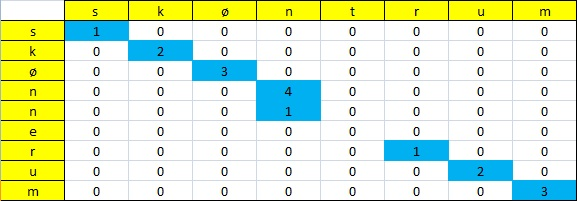
\includegraphics[scale=0.75]{figures/LcsExplained}
	\caption{An example of how two words are compared in LCS. The fields in yellow are the two words broken into characters ('Skøntrum' and 'Skønnerum'). The fields in blue indicates when LCS finds a match, the number indicates the length of the substring. In this case, LCS finds three sub strings:'skøn', 'n' and 'rum', the longest of the three is the first, and this will be the result that LCS returns to the user. }
	\label{LcsExplained}
\end{figure}

I will use the basic implementation of this algorithm in my thesis, I will then try and modify it to work better in context with finding article duplicates, instead of just the longest common substring.

\textbf{Problem:} This algorithm is very prone to fail in cases where there have been made alterations to the article in question. A word change in the middle of one of two otherwise identical articles will result in a ~50 \% match. If the article in question have been obfuscated with many changed words, the LCS will be extremely short. This is a high risk problem, as article duplication will often involve changing words. This algorithm is also substantially slower than the Cosine algorithm, having an O-notation of O(n*m). Ideally this algorithm is therefore best used on a selection of articles, rather than on the entire corpus.


\section{Optimizing Performance}
\subsection{Stop Words}
Stop word\footnote{\url{http://en.wikipedia.org/wiki/Stop_words}} removal would improve running time (performance) of both algorithms, and would pose little threat of causing either algorithm to fail (finding false positives). The exception to this could be very short articles (like breaking news articles\footnote{Breaking News articles is a thing of the 2000s. With the spread of media onto the Internet, an article is no longer a static printed piece of news in a paper. News can be published instantly on the web, and then updated as information are received. How ever, Breaking News articles can still be printed in the paper article with only little text attached to it.}), that only contains common words, like "Man walks away". Depending on the stop word list, this article could end up being \textit{null\footnote{An article with no text data.}}.
We can safely (with respects to the previously addressed problem) remove stop words, as they don't provide any \textit{semantic\footnote{\url{http://en.wikipedia.org/wiki/Semantics}}} value to the text.

\subsubsection{Cosine}
For the cosine algorithm removal of stop words would improve performance, by reducing the size of the \textit{Magnitude Vector}. 

\subsubsection{LCS}
In regards to the LCS algorithm, the performance would also be improved, as the algorithm wouldn't need to traverse as many characters. This would reduce the length of the longest common substring, but it would be unlikely that it would affect the outcome of the algorithm, as stop words are rarely changed when duplicating articles.

\subsection{Stemming}
\textit{Stemming}\footnote{\url{http://en.wikipedia.org/wiki/Stemming}} Stemming is the act of conjugating a word to the base form (Danish:\textit{'Grundform'}). It is done in order to reduce the amount of noise in a text. Words will then be conjugated and instead of having the same word represented several time in different conjugations they will all be noted as the same word. Stemming does not ruin the semantic content of the text.

\subsubsection{Cosine}
Stemming improves the performance of the cosine algorithm as this will reduce the number of words in the \textit{vector space}. As words would be reduced to their base form (Danish:\textit{Grundform}), words used several times, but with different endings would be counted as the same word. When using weighed evaluation this would actually improve performance to some extend. It can have a slight impact of the Cosine algorithm. This is because that without stemming the same word can occur several times in a text in different conjugations, and thus each conjugation would have a larger vector than when the conjugations are all counted as the same word. This impact will be minimal because the rare words are still occurring less often than normal words (stop words).

\subsubsection{LCS}
Stemming would not improve the performance of the LCS algorithm by much. As this algorithm matches characters one by one, it would make little difference if the words are stemmed or not. As the 'Grundform' is the shortest form of a word in Danish, it will make a slight difference, but this is hardly worth noting.

\section{Semaphore Tagging}
Another way of finding duplicates is by looking at each articles semaphore tags. When Infomedia receives articles in the inflow, these articles are enriched with \textit{Semaphore Tags}\footnote{Semaphore tags are tags that describes the contents of the article, an article about financial fraud would contain the tag \textit{Economic Crime}. These tags are created by the Infomedia Ontology (\url{http://en.wikipedia.org/wiki/Ontology_(information_science)}) team. They are creating rules for when a certain word (or words) appear in certain context, then an article will be tagged with a certain semaphore tag.}. A tag also has relations to other tags. A politician would be tagged with politics, political party, other people in politics that are in some way associated with that person. The tag is also enriched with a score, that is based on the relevance for that tag in that given article. So if a politician is the main focus of an article, the name of that politician is high than if the article deals with something that the politician only have a remote connection to. Each article then gets a number of tags based on what terms are found in the article. A way of finding article duplicates could be through creating an algorithm that would check a pair of articles with their respective semaphore tags.

\subsection{Cons to Semaphore}
As these tags are more of a general indicator to an articles' contents than an actual text matching algorithm, it will provide very little value as a stand alone implementation. Each article will only contain tags for the terms, for which the ontology team has created semantic rules for. If 100 articles all contained various doings of a minister (picking up the children, going to meetings, being involved in a crisis) many of the same tags would be present in the 100 articles, this could be the ministers name, political party and other general tags that are linked to this minister. It would therefore be hard to decipher much information that could truly and uniquely link two articles together just by doing this. However this could be used to enhance another algorithm (for instance one of the two mentioned above). If the articles compared contains the same tags, they are likely to have some sort of relevance to each other, and if the tags also have matching scores, that would strengthen the possibility of a match. I will not look any further into implementing this algorithm in this thesis, as this approach is difficult in providing a definite result.

\section{Text Preparation}
\label{TextPrep}
To reduce the chance of the algorithms failing in detecting duplicates, the text should be 'normalized'. As there are quite a few pitfalls in text analysis, one should try and take as many precautions as possible. A common source of error is common spelling errors, I will not check my article for spelling errors. These can have a rather big impact on the LCS algorithm. However as all text editors today have spell checking, this will be a tiny error source.

As the focus of this thesis have been on proving the thesis statement, there has been done no text preparation other than what is already implemented.

Another problem with text analysis is localized spelling. An example of this can be the Swedish town of Malmö. The issue here being the 'ö' letter which is in the Swedish alphabet. This town's name can be spelled in a few different ways.


\begin{itemize}
\item Malmö (Swedish spelling)
\item Malmø (Danish and Norwegian spelling)
\item Malmo (English spelling)
\item Malmoe (Phonetic spelling of the 'ö' character)
\end{itemize}

The same article could be in different newspapers, but with different spelling of the word. All words, or rather words containing special characters (non English characters) should therefore be normalized. In this case, the character 'ö' could be normalized into the letter 'o'. The phonetic spelling of the 'ö' character is highly unlikely to occur, as the normalized way of spelling 'Malmö' in languages without the 'ö' vowel, would be the third option. There is a lot of issues in this regard. This could be words or characters in a non Latin alphabet (Cyrillic, Arabic, Greek letters used in SI references or others). For this thesis, there is few non Danish texts or words in the test corpus, so it will have little influence. I will in this thesis not normalize text, but accept that minor deviance in scores can occur due to this.

Another good choice in text preparations is to lower case and remove all non alpha numerical characters. This can be advantageous for instance when looking at the name of the current Danish prime minister, Helle Thorning-Schmidt. As the hyphen can often be forgotten the last name can easily be misspelled. Removing the hyphen and replacing it with a blank space character would improve the accuracy of the algorithms. 

Stemming is another good way of normalizing text, I have already covered this topic in a previous section, and will not cover this more in detail here. 

Stop words will reduce the number of words in an article, and with less words, there are less error margin in terms of spelling errors, also less words in the article text means less words that has to be analysed. As stop words have little meaning when trying to figure out if two articles match, it is a good idea to remove these in order to improve performance. 

Unfortunately due to the time limit of this thesis, I will not be able to look into any of text the preparations mentioned, but wanted to describe what should be kept in mind, when implementing this project into Infomedia's inflow.

Finally it is important that all files are stored with the same encoding\footnote{\url{http://en.wikipedia.org/wiki/Character_encoding}}, as different encoding could cause havoc in the systems ability to read the text in the files. This is already done in the system, so I will not worry about this factor in my thesis.

\section{Technology}
As the inflow system at Infomedia is created in C$^\sharp$, it is the easy (and logical) choice to create my work in C$^\sharp$ as well. This would help integrating my work into the existing systems without too much trouble. I am using Visual Studio 2013 and .NET version 4.5 for my code development, which is provided to me by Infomedia. I am using Infomedias Team Foundation Server (TFS) for version control. 








                               	%Chapter 3
\appendix	
\chapter{Test Diagrams}

Examples of comparing two articles with LCS. More files can be found in the electronic appendixes.

\begin{sidewaysfigure}
	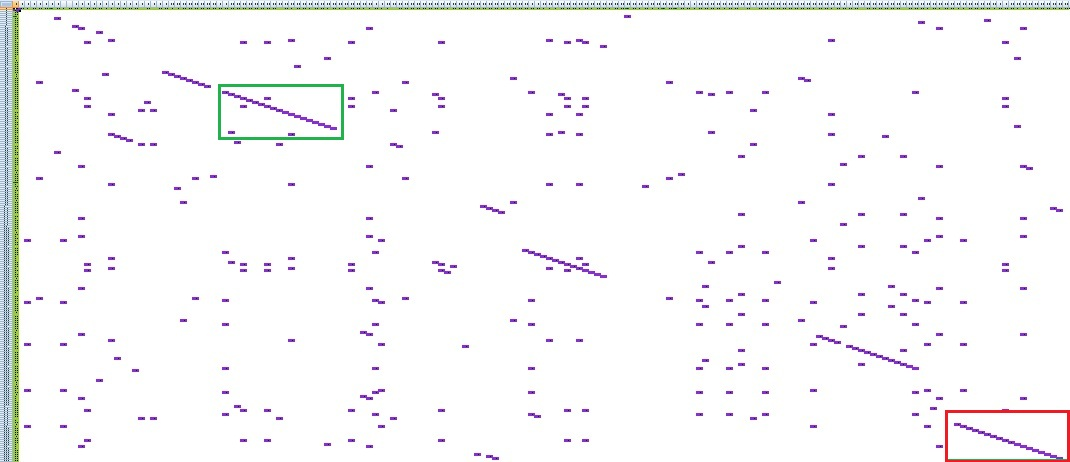
\includegraphics[scale=0.65]{figures/LcsExample}
	\caption{Diagram showing the result of two article being compared by using LCS.}
\end{sidewaysfigure}

\begin{sidewaysfigure}
	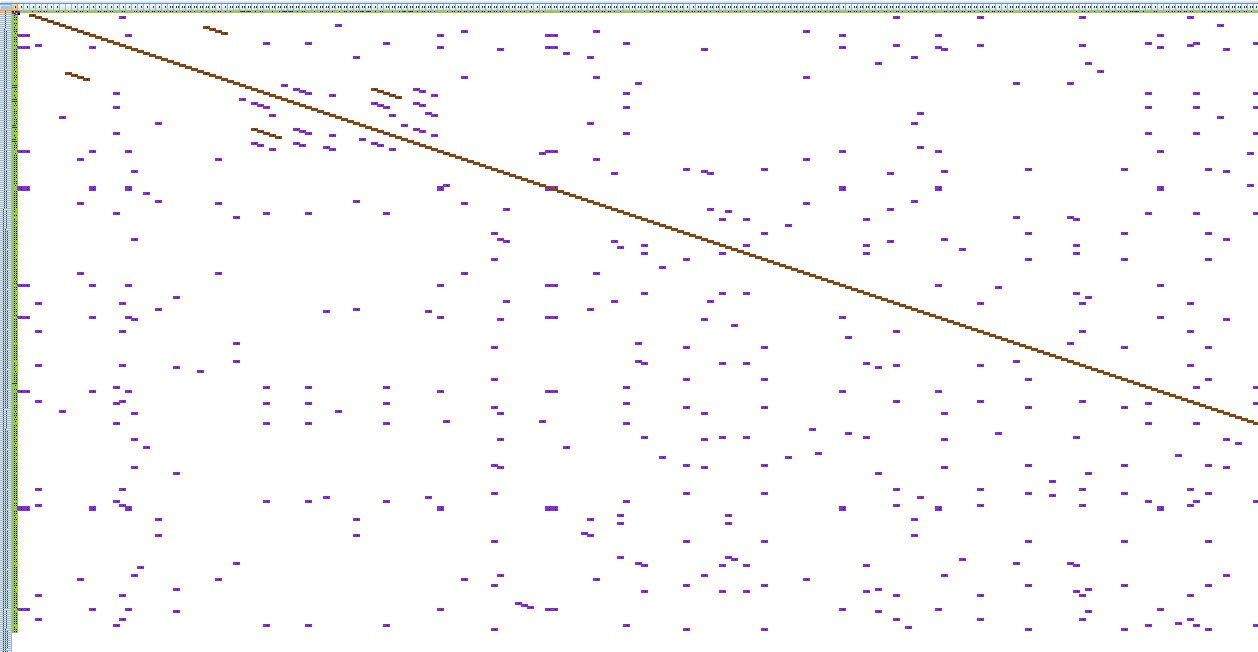
\includegraphics[scale=0.5]{figures/PerfectMatch}
	\caption{Diagram showing part of the result from running LCS on two articles that are almost a perfect match.}
\end{sidewaysfigure}

\begin{sidewaysfigure}
	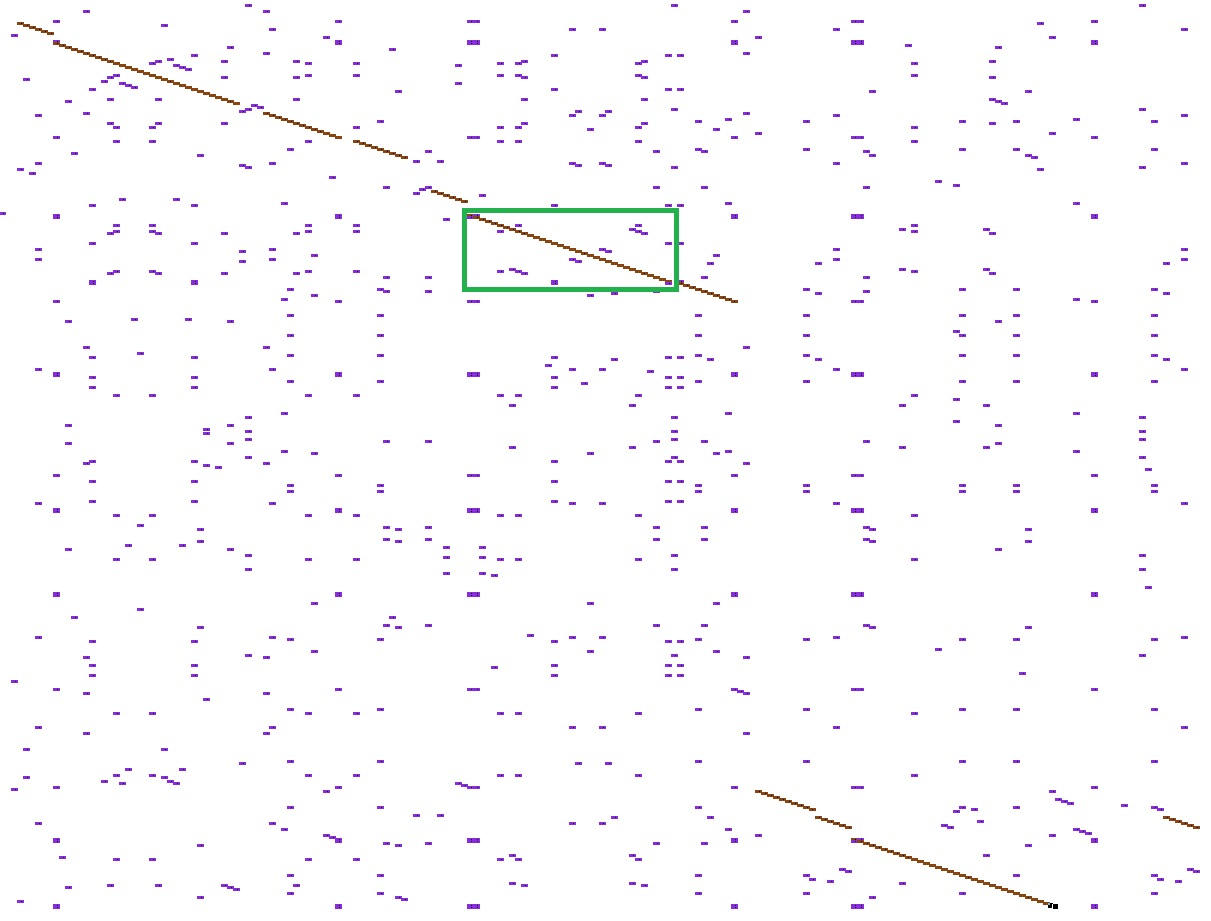
\includegraphics[scale=0.5]{figures/SubstringCollection}
	\caption{Diagram showing part of the result of running LCS on two articles and marking up all substrings with a length larger than three words.}
	\end{sidewaysfigure}                                 %Appendix A
%-----------
% Backmatter
%-----------
\backmatter
\chaptermark{Bibliography}
\renewcommand{\sectionmark}[1]{\markright{#1}}
\sectionmark{Bibliography}
\addcontentsline{toc}{chapter}{Bibliography}        %Force addition of Bibliography to TOC
\bibliographystyle{alpha}                           %Use alpha codes for references
\bibliography{References}                           %Bibliography file called
\end{document}
% % % EOF % % %